\section{OSTIA-Based Continuous Architecting}
This section elaborates on the ways in which OSTIA supports continuous
architecting. First, we elaborate on the anti-patterns supported in
OSTIA. Second, we elaborate on the algorithmic manipulation that OSTIA could
apply to topologies to provide alternative visualisation. Third, we discuss how
OSTIA suggests an alternative architecture to improve the system
performance. Fourth, finally, we elaborate on how OSTIA can drive continuous
improvement assisted by formal verification. All figures in these sections use a
simple graph-like notation where nodes may be any topological element (e.g.,
Spouts or Bolts in Apache Storm terms) while edges are directed data-flow
connections.


\subsection{Topology Design Anti-Patterns Within OSTIA}\label{sec:anti-pattern}
This section elaborates on the anti-patterns we elicited through self-ethnography. These anti-patterns are elaborated further within OSTIA to allow for their detection during streaming topology inference analysis. Every pattern is elaborated using a simple graph-like notation where \emph{spouts} are nodes that have outgoing edges only whereas \emph{bolts} are nodes that can have either incoming or outgoing edges respectively.

\subsubsection{Multi-Anchoring}
The Multi-Anchoring pattern is shown in Fig. \ref{fig:multi-anchoring}. In order to guarantee fault-tolerant stream processing, tuples processed by bolts need to be anchored with the unique id of the bolt and be passed to multiple acknowledgers (or ``ackers" in short) in the topology. In this way, ackers can keep track of tuples in the topology. Multiple ackers can indeed cause much overhead and influence the operational performance of the entire topology.
%\emph{\bf TODO: what is the consequence of these anti-patterns? How does OSTIA detect?}
%\emph{\bf Multi-anchoring is not supported at the moment. Besides, I am not sure it is an anti-patter but rather a design decision}

%\begin{figure}[H]
%	\begin{center}
%		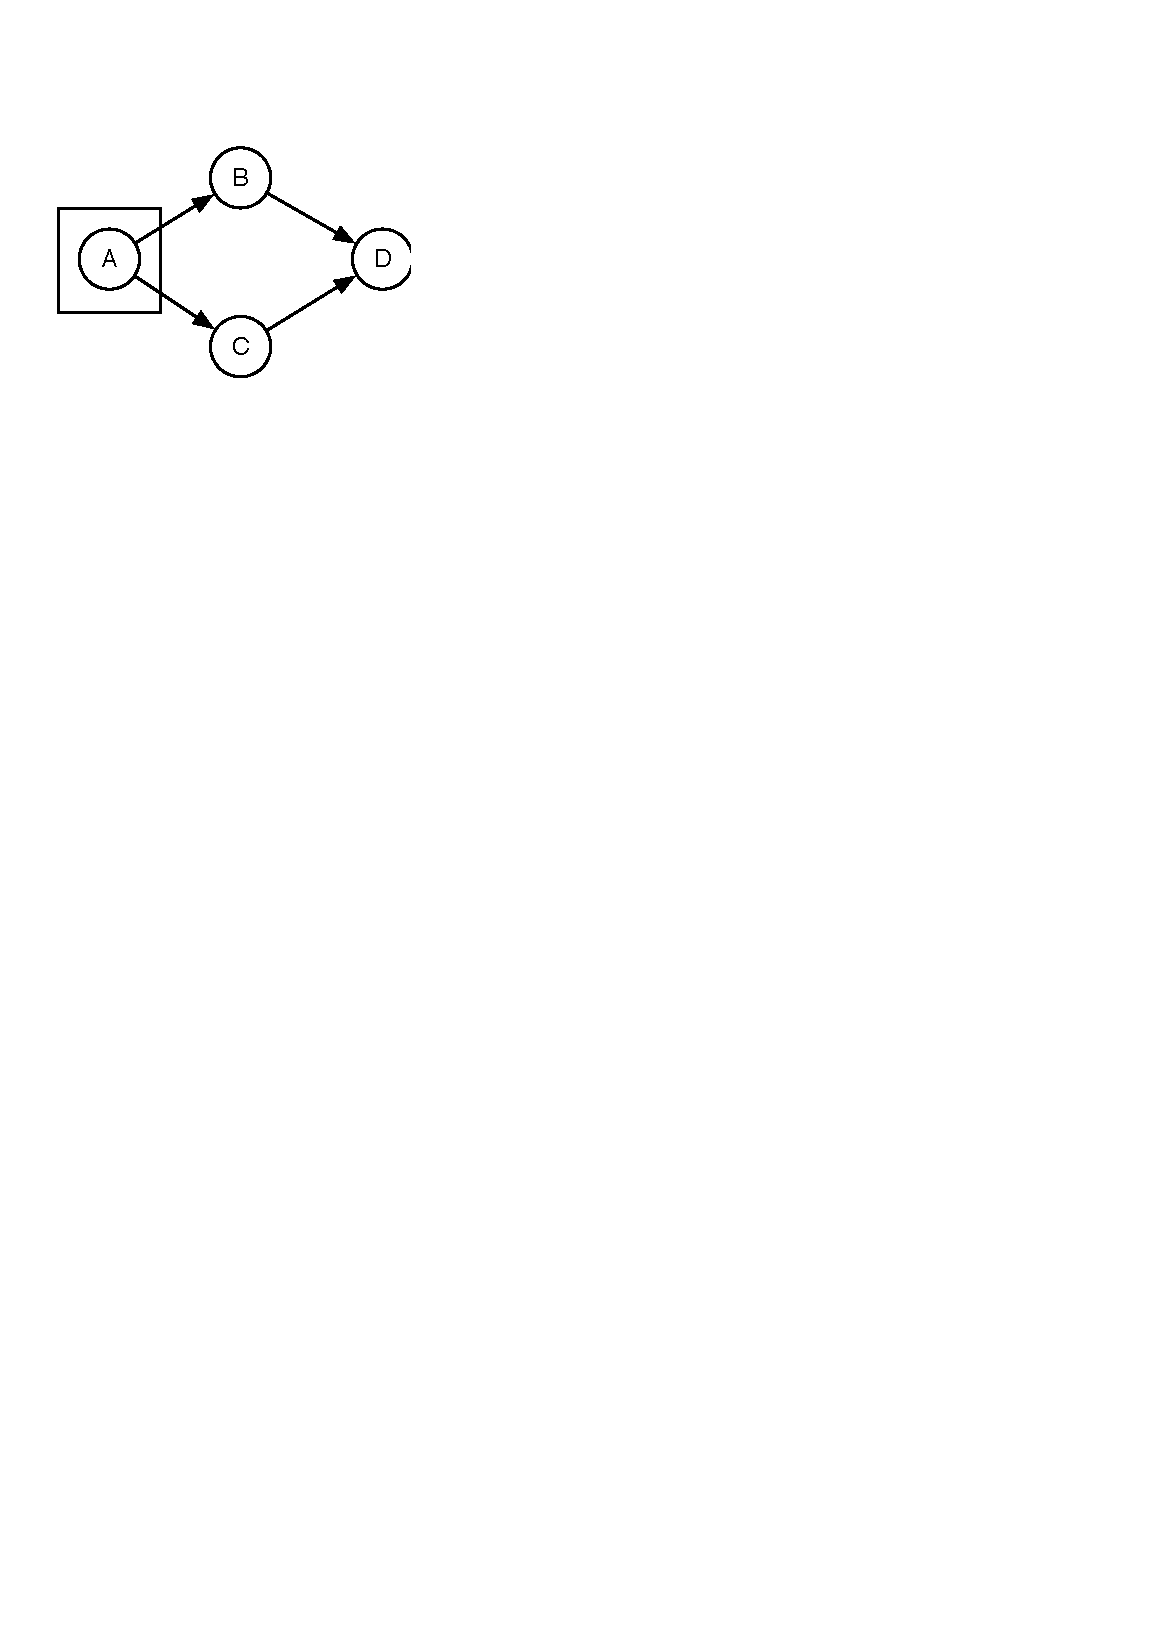
\includegraphics[width=2.5cm]{images/multi-anchoring}
%		\caption{Multi-anchoring.}
%		\label{fig:multi-anchoring}
%	\end{center}
%\end{figure}

\begin{figure}
\centering 
\subfigure[Multi-anchoring.]{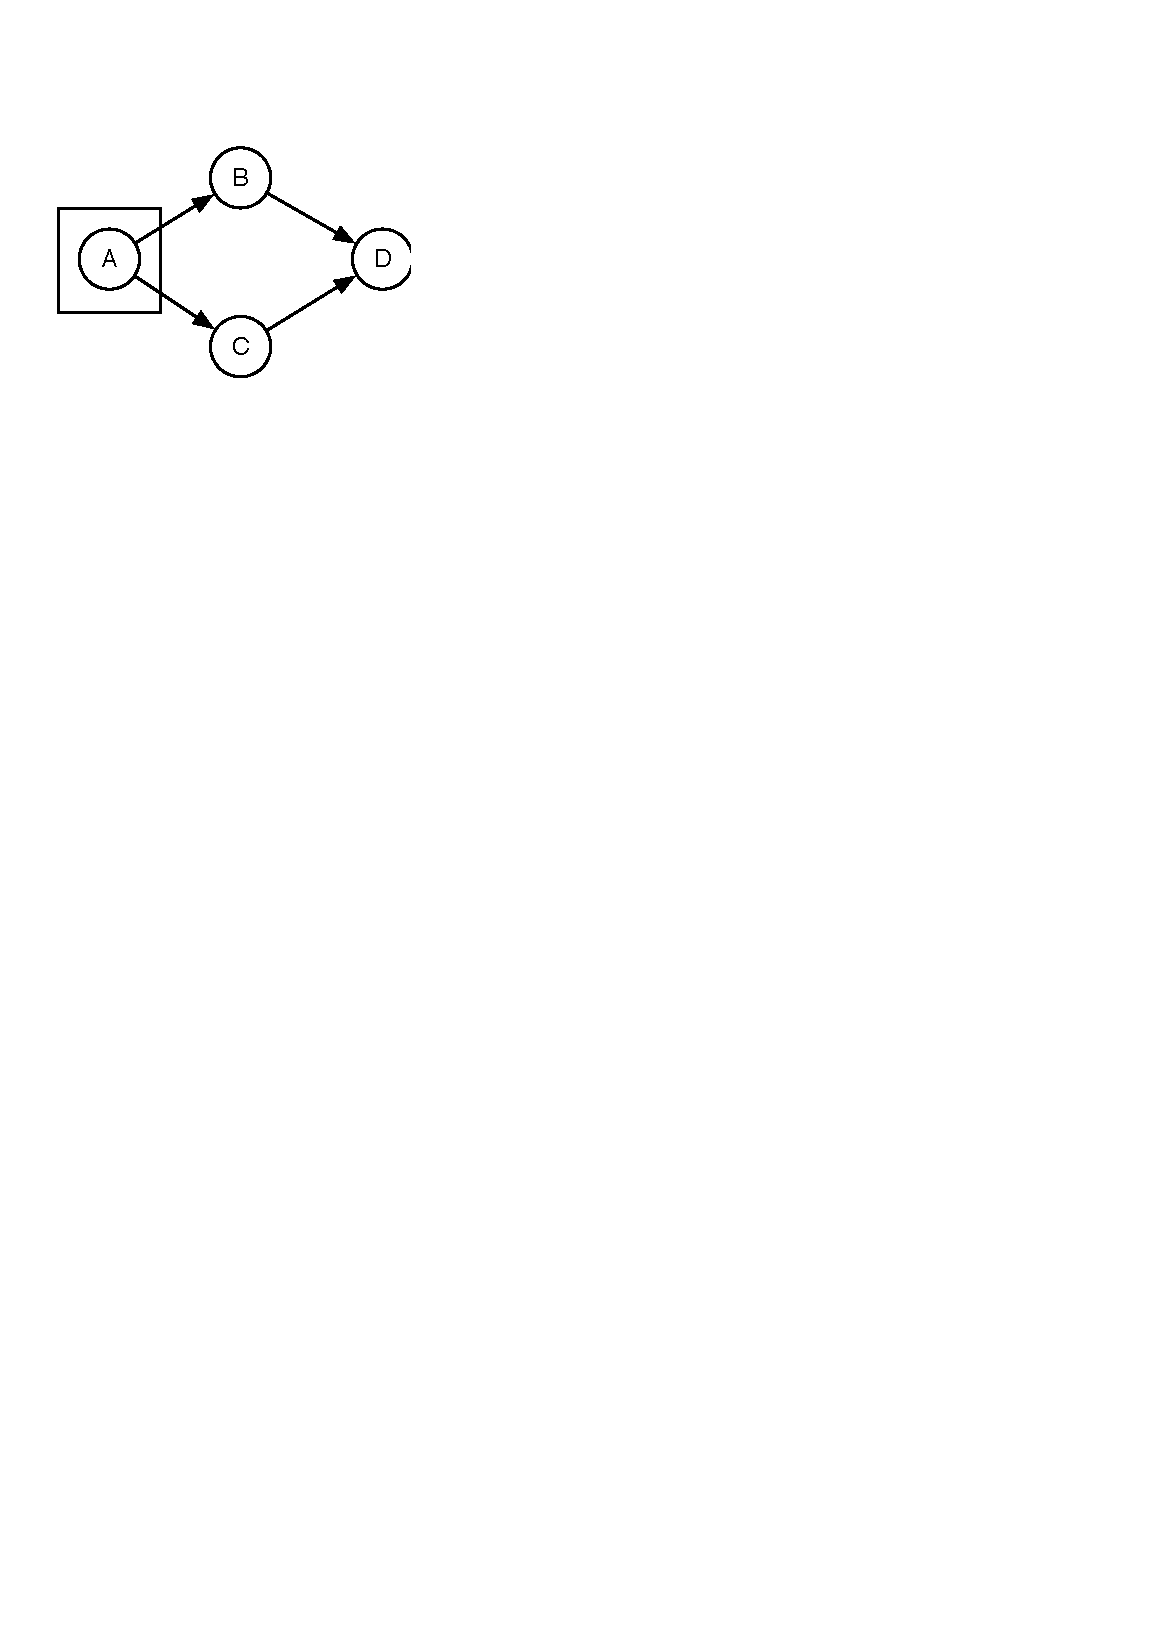
\includegraphics[width=3cm]{images/multi-anchoring}}\label{fig:multi-anchoring}
\hspace{1cm}
\subfigure[Cycle-in.]{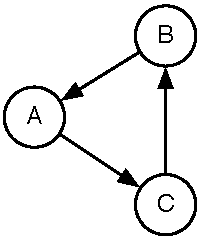
\includegraphics[width=2.5cm]{images/cycle}}\label{fig:cycle}
\end{figure}


\subsubsection{Cycle-in Topology}

The Cycle-in pattern is shown in Fig. \ref{fig:cycle}. Technically, it is possible to have cycle in Storm topologies. An infinite cycle of processing would create an infinite tuple tree and make it impossible for Storm to ever acknowledge spout emitted tuples. Therefore, cycles should be avoided or resulting tuple trees should be investigated additionally to make sure they terminate at some point and under a specified series of conditions. The anti-pattern itself may lead to infrastructure overloading and increased costs.
%\emph{\bf A topology is already an infinite stream of tuple, the problem could be the overloading of some machines}
%\emph{\bf At the cycle-detection is not supported (even if it is easy to implement)}

%\begin{figure}[H]
%	\begin{center}
%		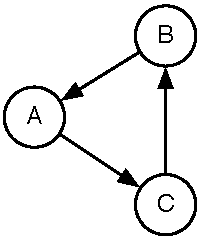
\includegraphics[width=2cm]{images/cycle}
%		\caption{Cycle-in Topology.}
%		\label{fig:cycle}
%	\end{center}
%\end{figure}

\subsubsection{Persistent Data}

The persistent data pattern is shown in Fig. \ref{fig:persistence}. This pattern covers the circumstance wherefore if two processing elements need to update a same entity in a storage, there should be a consistency mechanism in place. OSTIA offers limited support to this feature, which we plan to look into more carefully for future work. More details on this support are discussed in the approach limitations section.
%\emph{\bf Ostia does not support this. BTW is this static analysis? if not, is it off-topic?}

\begin{figure}
	\begin{center}
		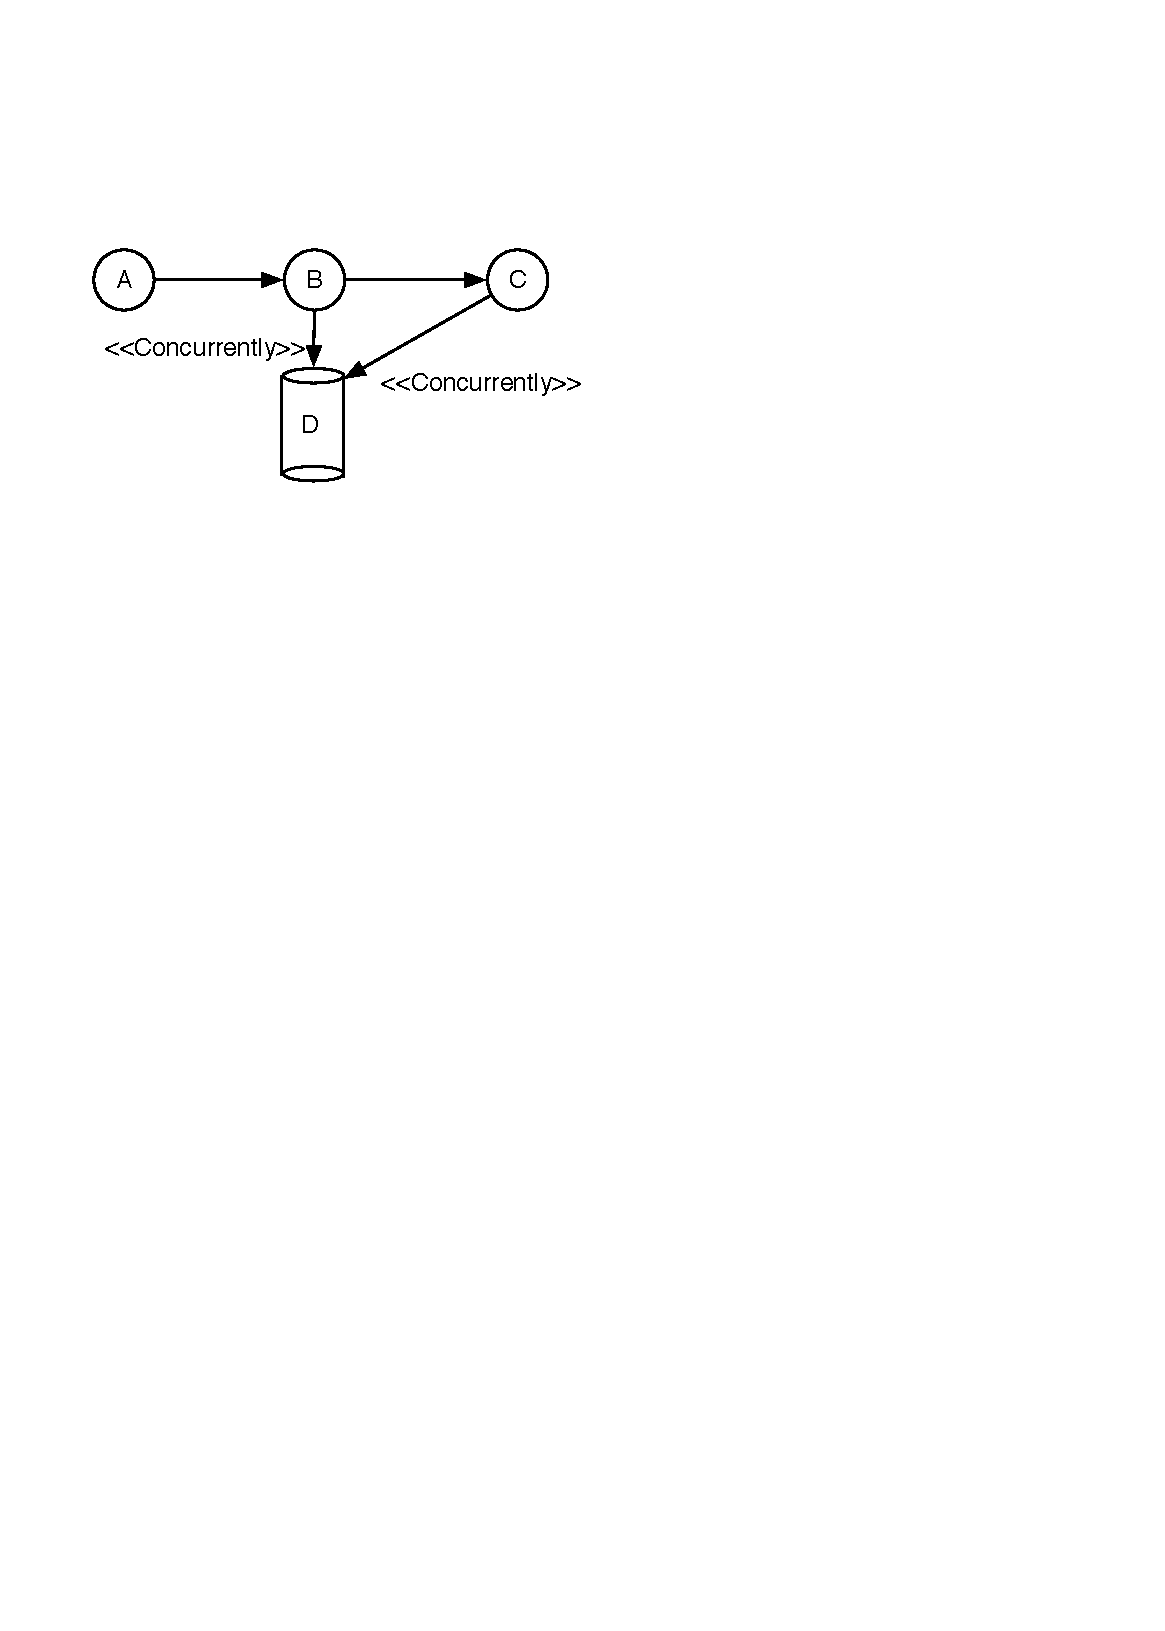
\includegraphics[width=5cm]{images/persistence}
		\caption{Concurrency management in case of Persistent Data circumstances.}
		\label{fig:persistence}
	\end{center}
\end{figure}


\subsubsection{Computation Funnel}
The computational funnel is shown in Fig. \ref{fig:funnel}. A computational funnel emerges when there is not a path from data source (spout) to the bolts that sends out the tuples off the topology to another topology through a messaging framework or through a storage. This circumstance should be dealt with since it may compromise the availability of results under the desired performance restrictions.

\begin{figure}
	\begin{center}
		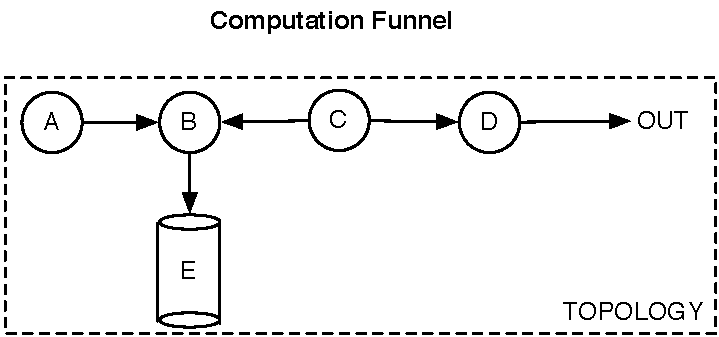
\includegraphics[width=6.5cm]{images/funnel}
		\caption{computation funnel.}
		\label{fig:funnel}
	\end{center}
\end{figure}

\subsection{Algorithmic Analysis on Stream Topologies}\label{algo}

This section elaborates on the algorithmic analysis supported by OSTIA using the common graph-like notation introduced previously. OSTIA currently supports two topology content analysis (see Sec. \ref{1} and \ref{2}) as well as two topology layout analyses (see Sec. \ref{3} and \ref{4}). Only a part of these analyses is currently implemented in OSTIA. We discuss approach limitations further in Sect. \ref{disc}.

\subsubsection{Fan-in/Fan-out}\label{1}

The Fan-in/Fan-out algorithmic manipulation is outlined in Fig. \ref{fig:fan}. For each element of the topology, fan-in is the number of incoming
streams. Conversely, fan-out is the number outgoing streams. In the case of
bolts, both in and out streams are internal to the topology. For Spouts,
incoming streams are the data sources of the topology (e.g., message brokers,
APIs, etc).

\begin{figure}
	\begin{center}
		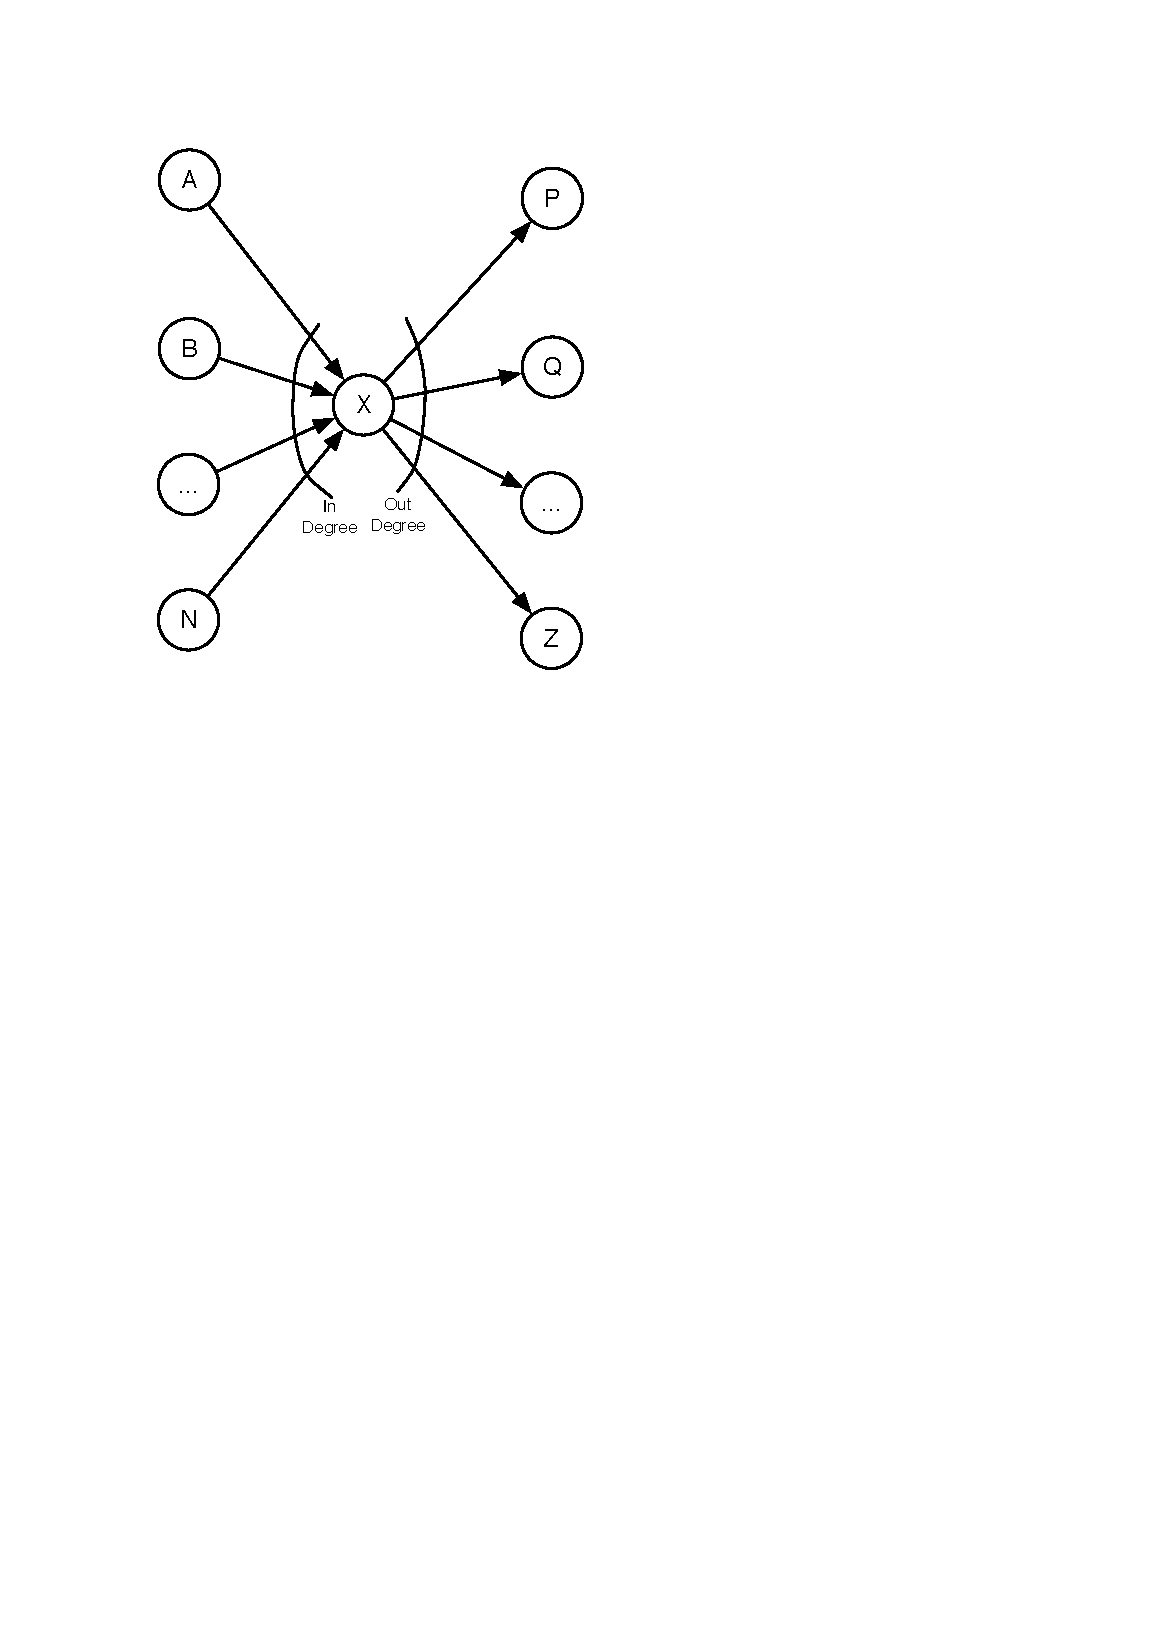
\includegraphics[width=3cm]{images/fan-in-out}
		\caption{Fan-in fan-out in Stream topologies.}
		\label{fig:fan}
	\end{center}
\end{figure}

This algorithmic manipulation allows to visualise instances where fan-in and fan-out numbers are differing.

\subsubsection{Topology cascading}\label{2}

The Cascading algorithmic manipulation is outlined in Fig. \ref{fig:cascading}. By topology cascading, we mean connecting two different Storm topologies via a messaging framework (e.g., Apache Kafka~\cite{kafka}).
%\footnote{\url{http://kafka.apache.org/}}). 
Although cascading may simplify the development of topologies by encouraging architecture elements' reuse especially for complex but procedural topologies, this circumstance may well raise the complexity of continuous architecting and may require separation of concerns \cite{soc}. For example, Fig. \ref{fig:cascading} outlines an instance in which two topologies are concatenated together by a message broker. In this instance, formal verification may be applied on the left-hand side topology, which is more business-critical, while the right-hand side of the entire topology is improved by on-the-fly OSTIA-based analysis. Even though OSTIA support for this feature is still limited, we report it nonetheless since OSTIA was engineered to address multiple topologies at once. 
%More details on this and similar limitations are discussed in Section \ref{lim}.
%\emph{\bf Ostia does not support this. I can't think of an easy way to implement it}

\begin{figure}
	\begin{center}
		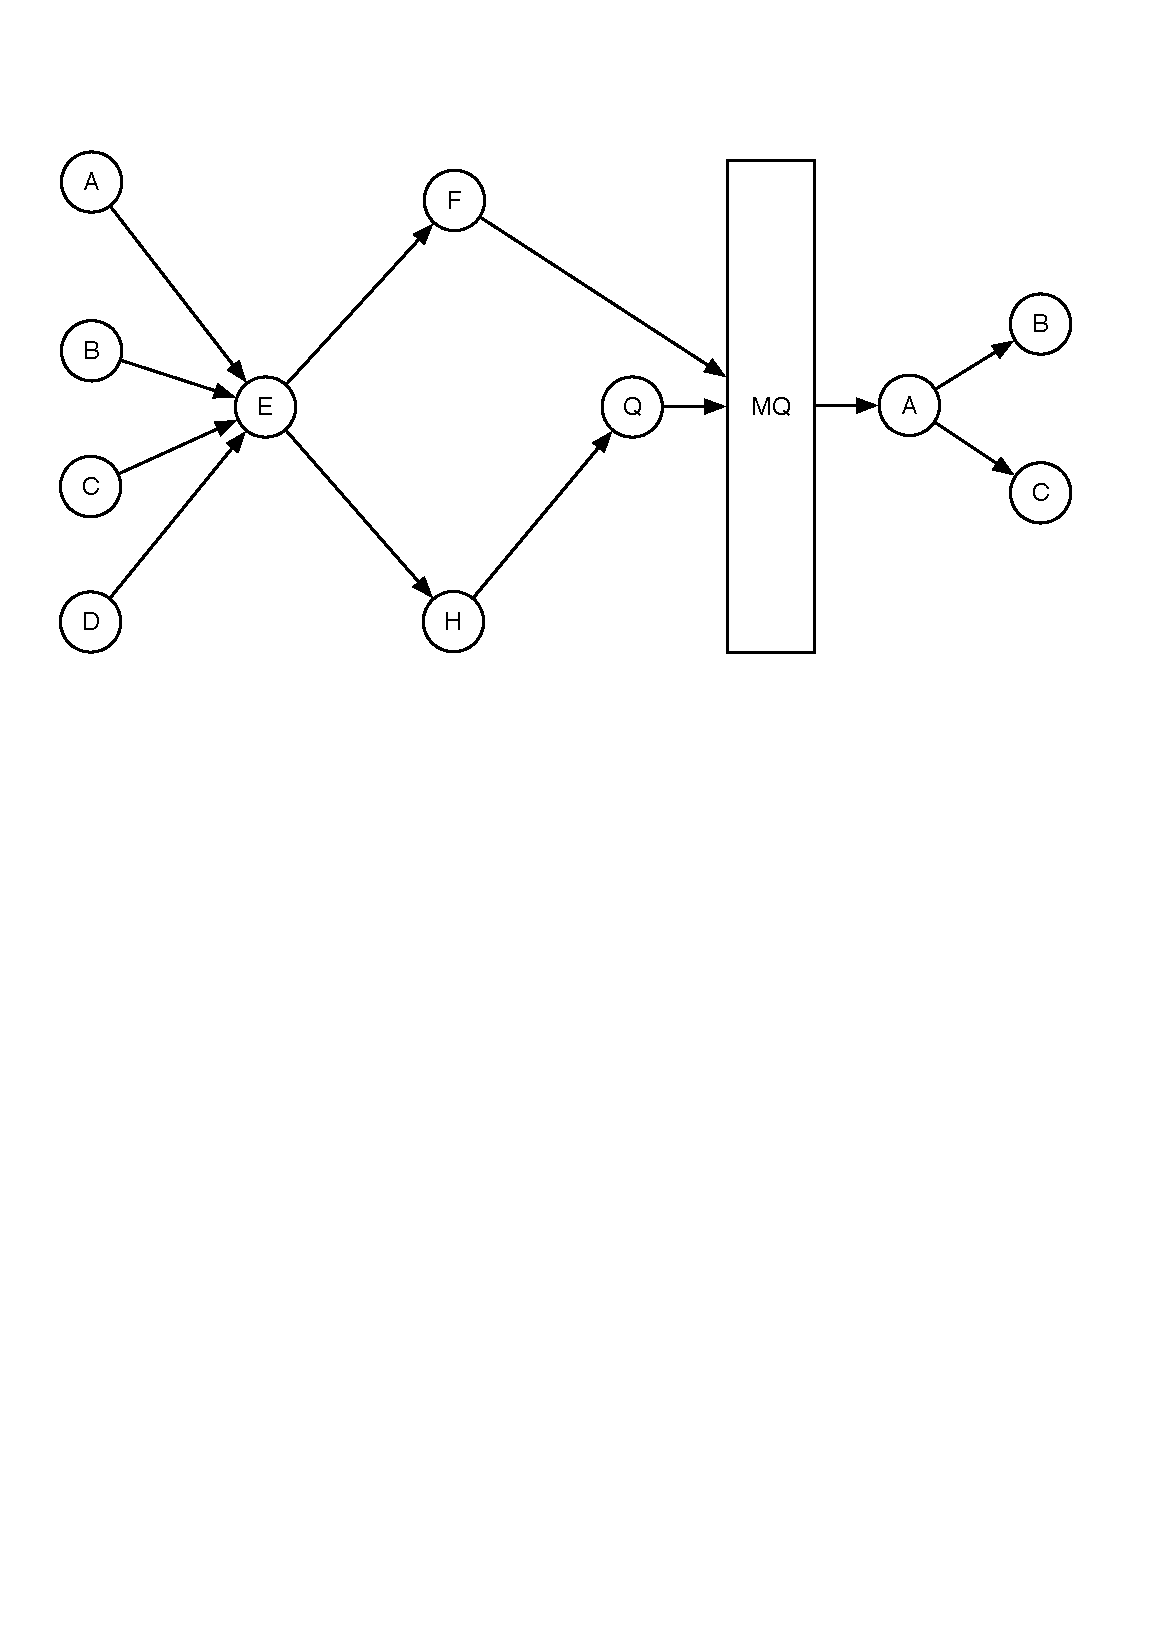
\includegraphics[width=6cm]{images/cascading}
		\caption{cascading.}
		\label{fig:cascading}
	\end{center}
\end{figure}

This algorithmic manipulation allows to combine multiple cascading topologies.

\subsubsection{Topology clustering}\label{3}
Topology clustering is outlined in Fig. \ref{fig:clustering}. Topology clustering implies identifying coupled processing elements (i.e., bolts and spouts) and cluster them together (e.g., by means of graph-based analysis) in a way that elements in a cluster have high cohesion and loose-coupling with elements in other clusters. Simple clustering or Social-Network Analysis mechanisms can be used to infer clusters. These clusters may require additional attention since they could turn out to become bottlenecks. Reasoning more deeply on clusters and their resolution may lead to establishing the Storm scheduling policy best-fitting with the application.
%\emph{\bf Does it relates with Storm scheduling?}

\begin{figure}
	\begin{center}
		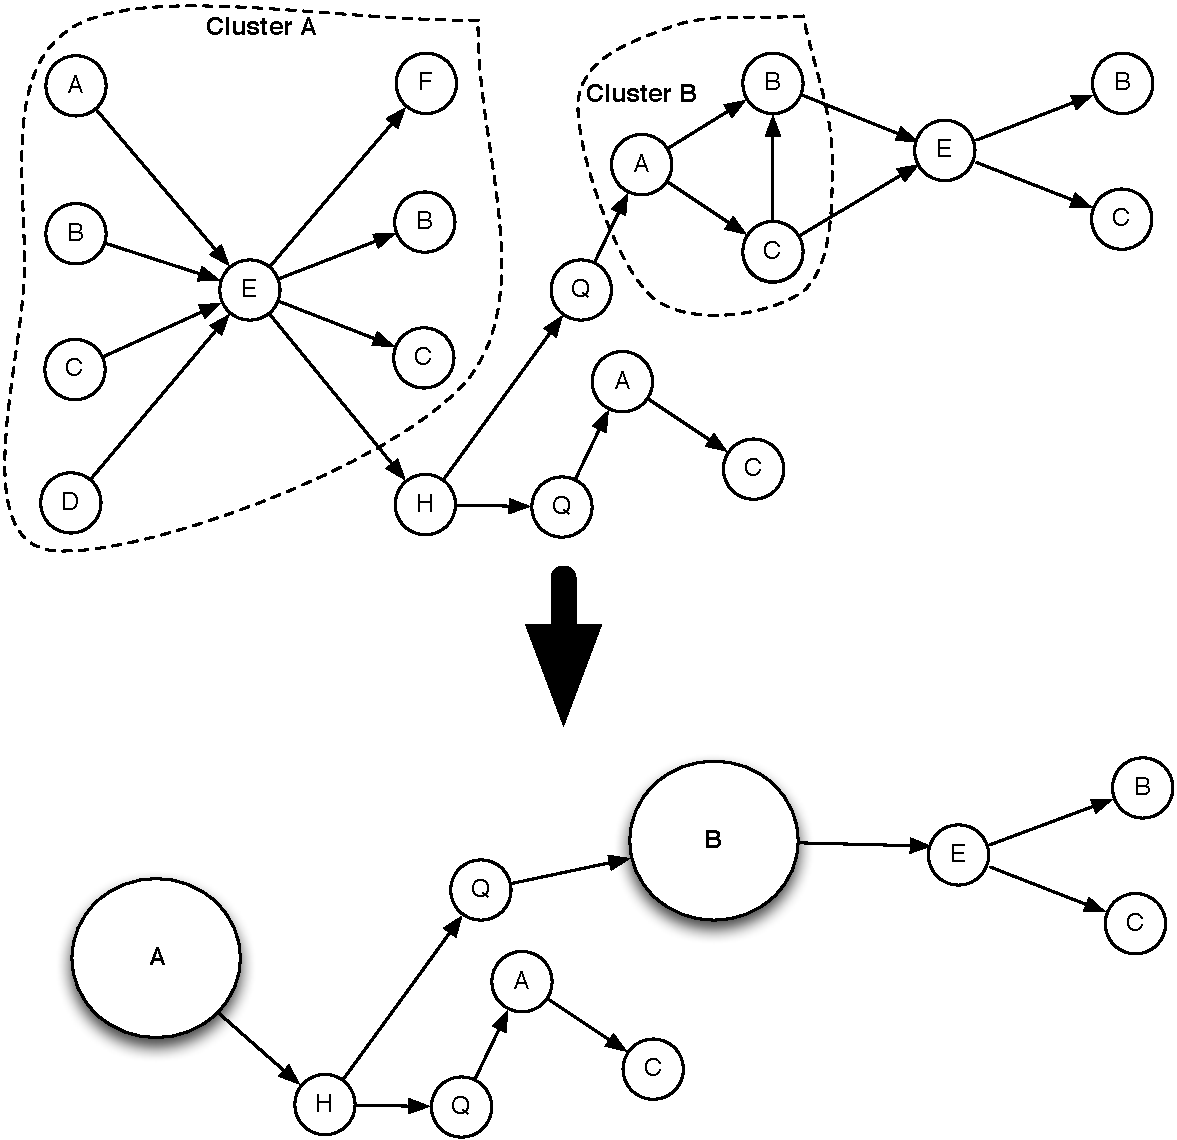
\includegraphics[width=6.5cm]{images/clustering}
		\caption{clustering.}
		\label{fig:clustering}
	\end{center}
\end{figure}

\subsubsection{Linearising a topology}\label{4}

Topology linearisation is outlined in Fig. \ref{fig:linearizing}. Sorting the processing elements in a topology in a way that topology looks more linear, visually. This step ensures that visual investigation and evaluation of the structural complexity of the topology is possible by direct observation. It is sometimes essential to provide such a visualisation to evaluate how to refactor the topology as needed.

\begin{figure}
	\begin{center}
		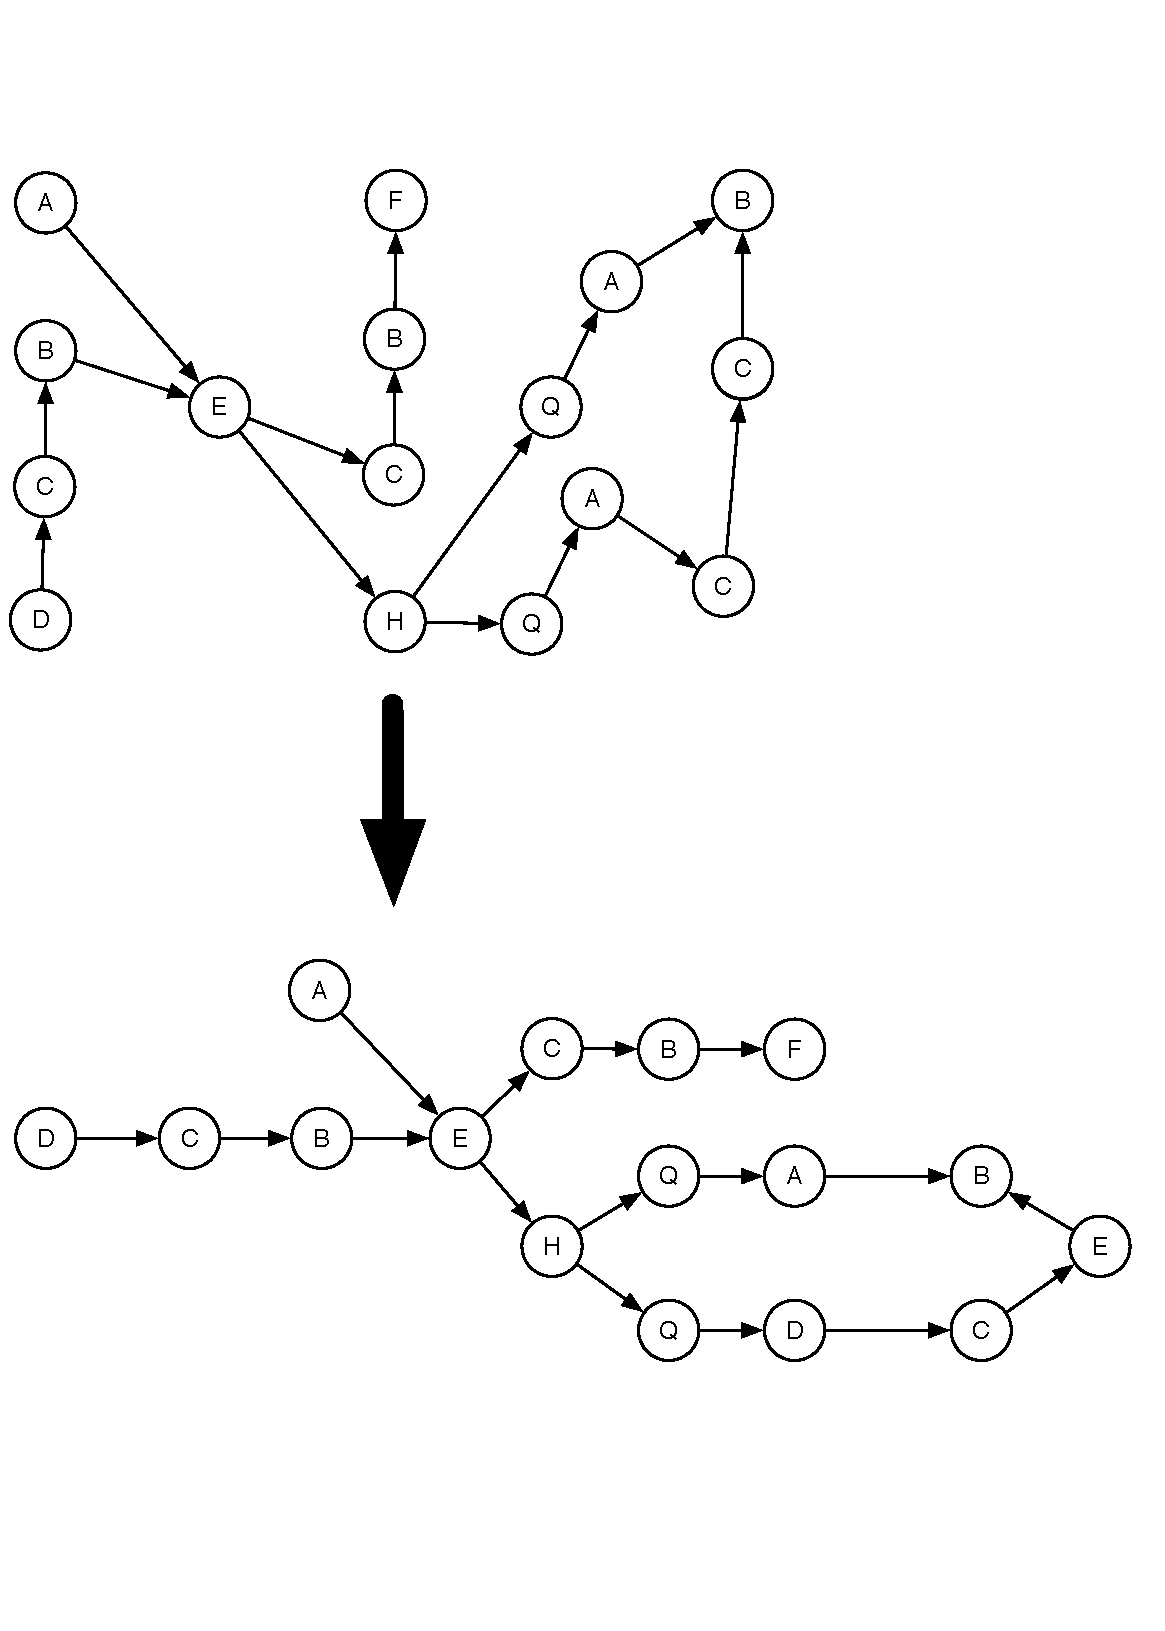
\includegraphics[width=5cm]{images/linearizing}
		\caption{linearising.}
		\label{fig:linearizing}
	\end{center}
\end{figure}

\subsection{Suggestions for Performance Improvements}
\label{sec:performance-boosting}

Big data architectures typically need parameters tuning to achieve best
performance. For instance, in Storm developers have to specify the parallelism
level for each node, which is the number of processes instantiated for a
particular bolt or spout. OSTIA provides suggestions on how to change the
parallelism level of the nodes, using simple and fast heuristics together with
static analysis.

After architects designed a Storm application, a scheduler instantiate the
topology on a cluster of machines. The default scheduler utilises a round-robin
strategy to fairly load the machines with the bolts and spouts. This a crucial
assumption for the heuristic used in OSTIA to perform well. There has been some proposal to change the default scheduler logic \comment{Andrea I added this sentence but please add some citations here} in order to boost the performance of the topologies, however, many Storm users typically prefer the default scheduler while having the opportunity to tune the parameter automatically behind the scenes.

The heuristic works as follow. A Storm architect runs OSTIA specifying the
number of machines used in the deployment and the number of instances of spouts
and bolts that can be spawned in each machine. OSTIA statically analyses the
topology and extract the parallelism level for each component of the
topology. At this point, we sum of all instances need to be allocated and the
slots available on the machines ($machines * components\_for\_each\_machine$).

OSTIA decides whether a possible improvements is possible (i.e. \emph{slots
  available} $>$ \emph{instances to be allocate}), and suggests changes to the
parallelism level to the nodes in order to improve the performance. The simplest
case occur when the unallocated slots are enough to remove a machine from the
cluster, thus saving costs.

Alternatively, OSTIA identify a subset of nodes, called critical nodes, which
are important from a performance perspective. The critical nodes of a topology
are defined as the nodes with the highest \emph{weighted fan-in}. The
\emph{weighted fan-in} of a node \emph{N} is defined by Equation \ref{eq:wfi}.

\begin{align}
  \text{weighted fan-in(N)} = \frac{\sum_{X \rightarrow N \in Edges} parallelism(X)}{parallelism(N)} \label{eq:wfi}
\end{align}

The critical nodes could be easily susceptible to overloading as their
parallelism level do not compensate the parallelism level of its
\emph{in-nodes}. Increasing the parallelism level gives the nodes more resources
to cope with high loads.

For instance, let us take Figure \ref{topo1} as an example. There are 22
components that needs to be allocated. Suppose that our cluster is composed by 4
machines and each machine fits 10 instances of components. OSTIA in this case
would suggest to simply remove one machine. Let us suppose that we have 3
machines with 10 tasks each. At this point we have 30 slots available and 22
components, therefore we have 8 slots available that can be used to increase the
performance. In order to decide the components to improves we identify the ones
with maximum \emph{weighted fan-in}. In the example nodes \emph{mediaExtractor}
and \emph{articleExtractor} with \emph{weighted fan-in} of 8. Finally, since we
have 8 free slots to share between two nodes we increase the parallelism level
of the two critical nodes of $8/2 = 4$, setting it from 1 to 5.

\comment{I really liked the section but I think if we can find a way to link this up with the verification somehow and evaluate this would be perfect, can Francesco do this?}

\subsection{OSTIA-Based Formal Verification}\label{ver}

\newcommand{\I}{\mathcal{I}}
\newcommand{\M}{\mathcal{M}}
\newcommand{\timestr}{\mathcal{T}}

\newcommand{\D}{\mathcal{D}}
\newcommand{\C}{\mathcal{C}}

%old, compatibility reasons
\newcommand{\U}{\mathbf{U}}
\newcommand{\Snc}{\mathbf{S}}
\newcommand{\T}{\mathbf{T}}
\newcommand{\R}{\mathbf{R}}

\newcommand{\Nat}{\mathbb{N}}
\newcommand{\Z}{\mathbb{Z}}
\newcommand{\Real}{\mathbb{R}}
\newcommand{\Q}{\mathbb{Q}}

%old, compatibility reasons

\newcommand{\X}[1]{\mathbf{X}\left(#1\right)}
\newcommand{\Y}[1]{\mathbf{Y}\left(#1\right)}

%\newcommand{\X}{\mathbf{X}}
%\newcommand{\Y}{\mathbf{Y}}


\newcommand{\Zed}{\mathbf{Z}}
\newcommand{\Lng}{\mathscr {L}}
\newcommand{\iFF}{\Leftrightarrow}
\newcommand{\niFF}{\nLeftrightarrow}
\newcommand{\SNC}{{\mathcal S}}
\newcommand{\TRG}{{\mathcal T}}
\newcommand{\zot}{$\mathds{Z}$ot}
%old, compatibility reasons
\newcommand{\G}[1]{\mathbf{G}\left(#1\right)}
\newcommand{\F}[1]{\mathbf{F}\left(#1\right)}
%\newcommand{\Q}{\mathbb{Q}}

\newcommand{\triple}[3]{(#1, #2, #3)}
\newcommand{\pair}[2]{(#1, #2)}
\newcommand{\siff}{\Leftrightarrow}
\newcommand{\A}{\mathcal{A}}
\newcommand{\aX}{\mathrm{X}}
\newcommand{\aY}{\mathrm{Y}}
\newcommand{\x}{\mathbf{x}}
\newcommand{\eqdef}{\stackrel{\mbox{\begin{tiny}def\end{tiny}}}{=}} % =def=
\newcommand{\iFFdef}{\stackrel{\mbox{\begin{tiny}def\end{tiny}}}{\iFF}}
% =def=
\newcommand{\step}[1]{\xrightarrow{#1}}

\newcommand{\pspace}{\textsc{PSpace}}


\makeatletter
\def\Eqlfill@{\arrowfill@\Relbar\Relbar\Relbar}
\newcommand{\longmodels}[1][]{\,|\!\!\!\ext@arrow 0359\Eqlfill@{#1}}
\makeatother

\newcommand{\symodels}{\longmodels{\mbox{\it{\tiny sym}}}}

\newcommand{\intervaLii}[2]{[#1,#2]}
\newcommand{\intervaLie}[2]{[#1,#2)}
\newcommand{\intervaLee}[2]{(#1,#2)}

\newcommand{\interval}[2]{\langle #1,#2 \rangle}

\newcommand{\set}[1]{\{ #1 \}}

\newcommand{\tsys}[1]{\mathcal{S}(#1)}


\newcommand{\lapp}[1]{\lfloor #1 \rfloor}
\newcommand{\happ}[1]{\lceil #1 \rceil}


\newcommand{\first}[2]{(H_{#1}\vee L_{#1}) \wedge(\neg(H_{#1}\vee L_{#1}) \Snc (#2))}



\newcommand{\pname}[1]{\ensuremath{\textit{#1}}}
\newcommand{\on}{\pname{on}}
\newcommand{\off}{\pname{off}}
\newcommand{\lon}{\pname{l}}
\newcommand{\test}{\pname{test}}
\newcommand{\resetc}{\pname{reset-c}}
\newcommand{\turnoff}{\pname{turnoff}}




\newcommand{\edge}[1]{\texttt{#1}}
\newcommand{\enabled}[1]{\texttt{e}_{#1}}

\newcommand{\visit}[1]{\mathit{visit}(#1)}
\newcommand{\inv}[1]{\mathit{inv}(q_{#1})}


\newcommand{\intg}[1]{\lfloor#1\rfloor}
\newcommand{\fract}[1]{\mathit{frac(#1)}}



%%%%%%%%%%%%%%% STORM MODEL COMMANDS


\newcommand{\ori}{\mathtt{orig}}
%commands with single parameter
\newcommand{\p}[1]{\mathtt{process}_{#1}}
\newcommand{\ta}[1]{\mathtt{take}_{#1}}
\newcommand{\e}[1]{\mathtt{emit}_{#1}}
\newcommand{\add}[1]{\mathtt{add}_{#1}}
\newcommand{\f}[1]{\mathtt{fail}_{#1}}
\newcommand{\buf}[1]{\mathtt{buffer}_{#1}}
\newcommand{\startf}[1]{\mathtt{startFailure}_{#1}}
\newcommand{\startid}[1]{\mathtt{startIdle}_{#1}}
\newcommand{\id}[1]{\mathtt{idle}_{#1}}
\newcommand{\cl}[1]{\mathtt{clock}_{#1}}
\newcommand{\cltf}[1]{ \cl{to\f{#1}}}
\newcommand{\ph}[1]{\mathtt{phase}_{#1}}

%commands with two parameters (index, rate)
\newcommand{\pr}[2]{\p{#1}(#2)}
\newcommand{\tar}[2]{\ta{#1}(#2)}
\newcommand{\er}[2]{\e{#1}(#2)}
\newcommand{\addr}[2]{\add{#1}(#2)}
\newcommand{\ra}[1]{r_{\add{#1}}}
\newcommand{\rp}[1]{r_{\p{#1}}}
\newcommand{\re}[1]{r_{\e{#1}}}
\newcommand{\rt}[1]{r_{\ta{#1}}}
\newcommand{\rf}[1]{r_{\mathtt{failure}_{#1}}}
\newcommand{\rff}[2]{r_{\mathtt{failure}_{#1#2}}}
\newcommand{\rr}[1]{r_{\mathtt{replay}_{#1}}}
\newcommand{\reb}[1]{\bar{r}_{\e{#1}}}
\newcommand{\rth}[1]{\hat{r}_{\ta{#1}}}
\newcommand{\reh}[1]{\hat{r}_{\e{#1}}}

\newcommand{\tph}[2]{t_{\ph{#1}}^{#2} }

	

This section describes the formal modelling and verification employed in OSTIA. Our assumption for continuous architecting, is that architects eliciting and studying their topologies by means of OSTIA may want to continuously and incrementally improve it based on results from solid verification approaches. The approach we outline, relies on \textit{satisfiability checking}~\cite{MPS13}, an alternative approach to model-checking where, instead of an operational model (like automata or transition systems), the system (i.e., a topology in this context) is specified by a formula defining its executions over time and properties are verified by proving that the system logically entails them.

%The logic we use is Constraint LTL over clocks 
CLTLoc is a real-time temporal logic and, in particular, a semantic restriction of Constraint LTL (CLTL)~\cite{DD07} allowing atomic formulae over $(\mathbb{R}, \set{<,=})$ where the arithmetical variables behave like clocks of Timed Automata (TA)~\cite{timed}.
A clock $x$ measures the time elapsed since the last time when $x=0$ held, i.e., since the last ``reset'' of $x$.
Clocks are interpreted over Reals and their value can be tested with respect to a positive integer value.
%
Let $X$ be a finite set of clock variables $x$ over $\Real$, $Y$ be a finite set of variables over $\Nat$ and $AP$ be a finite set of atomic propositions $p$.
CLTLoc formulae with counters are defined as follows:
\begin{equation*}%\small
  \phi :=
  \begin{gathered}
    p \mid x\sim c \mid y\sim c\mid \aX y\sim z\pm c \mid\phi \wedge \phi \mid \neg \phi \mid \\
       \X{\phi} \mid \Y{\phi} %\mid \Zed\phi
\mid \phi\U\phi \mid \phi\Snc\phi
  \end{gathered}
\end{equation*}
where $x \in X$, $y,z \in Y$, $c \in \Nat$ and 
$\sim \in \set{<,=}$, $\bullet$, $\circ$, $\U$ and $\Snc$ are the
usual ``next'', ``previous'', ``until'' and ``since''.
%The semantics of CLTLoc is defined with respect to $(\Real, \set{<,=})$ and $\pair{\Nat}{<}$, the latter representing positions in time.
A \textit{model} is a pair $\pair{\pi}{\sigma}$, where $\sigma$ is a mapping associating every variable $x$ and position in $\Nat$ with value $\sigma(i,x)$ and $\pi$ is a mapping associating each position in $\Nat$ with subset of $AP$. 
The semantics of CLTLoc is defined as for LTL except for formulae $x\sim c$ and $\aX y \sim z\pm c$. 
%At position $i\in\Nat$, $ \pair{\pi}{\sigma}, i \models x\sim c \textbf{ iff }  \sigma(i, x)\sim c$ and $\pair{\pi}{\sigma}, i \models \aX y\sim z \pm c \textbf{ iff }  \sigma(i+1, z) \sim \sigma(i,z) \pm c$.
Intuitively, formula $x\sim c$ states that the value of clock $x$ is $\sim$ than/to $c$ and formula $\aX y \sim z\pm c$ states that the next value of variable $y$ is $\sim$ to/than $z+c$.

The standard technique to prove the satisfiability of CLTL and CLTLoc formulae is based on of B\"uchi automata \cite{DD07,BRS15} %the evidence has turned out that it may be rather expensive in practice, even in the case of LTL (the size of the automaton is exponential with respect to the size of the formula).
but, for practical implementation, Bounded Satisfiability Checking (BSC)~\cite{MPS13} avoids the onerous construction of automata by means of a reduction to a decidable Satisfiability Modulo Theory (SMT) problem~\cite{BRS15}.
%By unrolling the semantics of a formula for a finite number $k>0$ of steps, 
The outcome of a BSC problem is either an infinite ultimately periodic model or unsat.
%\cite{BRS15} shows that BSC for CLTLoc is complete and that is reducible to a decidable Satisfiability Modulo Theory (SMT) problem. 
%A CLTLoc formula can be translated into the decidable theory of quantifier-free formulae with equality and uninterpreted functions combined with the theory of Reals over $(\Real,<)$. %, written QF-EUF$(\Real,<)$.

CLTLoc allows the specification of non-deterministic models using temporal constraints wherein clock variables range over a dense domain and whose value is not abstracted.
Clock variables represent, in the logical language and with the same precision, physical (dense) clocks implemented in real architectures.
%They appear in formulae in the form $x \sim c$ to express a bound $c$ on the delay measured by clock $x$. 
Clocks are associated with specific events to measure time elapsing over the executions.
As they are reset when the associated event occurs, in any moment, the clock value represents the time elapsed since the previous reset and corresponds to the elapsed time since the last occurrence of the event associated to it.
We use such constraints to define, for instance, the time delay required to process tuples or between two node failures.\\

%Modeling topologies requires to express by formulae emitting rates which measure the number of tuples emitted by a spout node per time unit.
%***TBC

%Verification techinques:
%\begin{itemize}
%\item Safety Verification
%\item Performance analysis	
%\end{itemize}
%A \textit{safety} property is intuitively defined in the formal verification context as a property stating that something ``bad'' will \textit{never} happen during execution.\cite{lamport1}
%Cassical examples of safety properties are deadlock freedom and mutual exclusion, where the ``bad'' behaviour is respectively the deadlock occurrence and the simultaneous execution of a critical section.
%One of the most important requirements for streaming systems is guaranteeing low latency while maintaining high throughput. 
%In a distributed  --> Motivare questione delle code!
%

%
%\subsection{Storm Formal Model}
%\label{sec:storm-model}
%To perform our verification tasks we defined a formal model expressed in CLTLoc with discrete variables. The resulting model is a non-deterministic infinite state system.

% MOVED BEFORE
%%%\subsubsection{OSTIA Models: a Formal Interpretation}
%%%We started by understanding and capturing the behaviors of both spouts and bolts. 
%%%After choosing the level of abstraction of our model we simplified those behaviors accordingly, in order to formalize them as finite state machines. The purpose of this first activity was to define the possible operations and the allowed orderings of such operations.
%%%We then extended the model by taking into account the message buffers (or queues) and the quantity of tuples that are exchanged through the topology.
%%%In addition to the correct ordering of the operations, we decided to introduce more specific temporal constraints into the model, in order to limit the time spent by the system in each state (or processing phase) and to elaborate the concept of \textit{rate}, intended as ``number of times an event is occurring every time unit''.\\

%\subsubsection{Assumptions and  level of abstraction}
%We made several assumptions and abstractions while building the model:

Building on top of the above framework,  a formal interpretation of the Storm (meta-)model requires several abstractions and assumptions.

%For example, some deployment details, such as the number of worker nodes and features of the underlying cluster, are abstracted away. 
%There is a single queuing layer: every bolt has a unique incoming queue and no sending queue, while the worker queues are not represented. In the same way, each bolt/spout has a single output stream.
%Moreover, the content of messages is not relevant: all the tuples have the same fixed size and we represent only quantity of tuples moving through the system.


\begin{itemize}
	\item some deployment details, e.g., the number of worker nodes and features of the underlying cluster, are abstracted away;
	\item each bolt/spout has a single output stream;
	\item %we simplified the message buffer system, assuming that 
	there is a single queuing layer: every bolt has a unique incoming queue and no sending queue, while the worker queues are not represented;
	\item every operation is performed within minimum and maximum thresholds of time;
	\item %we do not take into account 
	the content of the messages is not relevant: all the tuples have the same fixed size and we represent only quantity of tuples moving through the system;
\end{itemize}

%\subsubsection{Model Formalization}
A Storm Topology is a directed graph $\mathbf{G} = \{ \mathbf{N}, Sub\}$ where the set of nodes $\mathbf{N} = \mathbf{S}\bigcup \mathbf{B}$ includes in the sets of spouts (\textbf{S}) and bolts (\textbf{B}) and %the set of edges $\mathbf{E} = \{ Sub_{i,j} | i \in \mathbf{B}, j \in \{\mathbf{S}\bigcup \mathbf{B}\} \}$ 
$Sub\subset\mathbf{N}\times\mathbf{N}$ defines how the nodes are connected each other via the subscription relation. Pair $(i,j)\in Sub$ indicates that ``bolt $i$ subscribes to the streams emitted by the spout/bolt $j$''. 
Spouts cannot subscribe to other nodes in the topology.
Each bolt has a receive queue where the incoming tuples are collected before being read and processed. % by the node.
The queues have infinite size and the level of occupation of each $j^{th}$ queue is described by the variable $q_j$. %\footnote{Spouts have no queues, by definition.}
Spouts have no queues, and 
each spout can either \textit{emit} tuples into the topology or stay \emph{idle}.
Each bolt can be in \emph{idle} state, in \emph{failure} state or in  \emph{processing} state.  While in the processing state, the bolt first reads tuples from its receive queue (\textit{take} action), then it performs its transformation (\textit{execute} action) and finally it \textit{emits} the output tuples in its output streams. \\
\begin{figure}[tb]
\centering
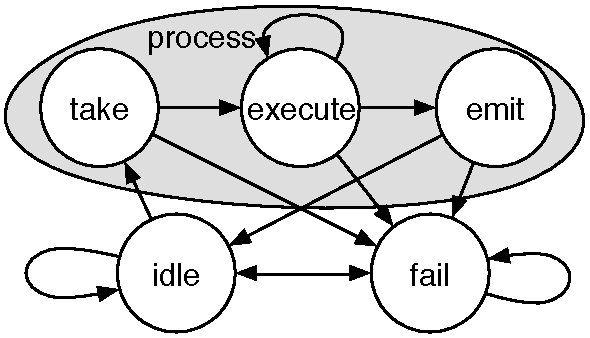
\includegraphics[width=0.7\linewidth]{images/bolt-fsm}
\caption{Finite state automaton describing bolt states.}
\label{figure-fsa}
\end{figure}

%\begin{figure}
%	\centering	
%	\begin{tikzpicture}[->,>=stealth',shorten >=1pt,auto,node distance=2.5cm,semithick, every node/.style={scale=0.55}]
%	
%	\tikzstyle{every state}=[fill=white,text=black,minimum width={width("execute")+10pt}]
%	
%	
%	\node[state]            (I) {$idle$};  
%	\node[state]         (T) [above right of=I] {$take$};  
%	\node[state]         (E) [right of=T] {$execute$};
%	\node[state]         (F) [below right of=I] {$fail$};
%	\node[state]         (EM) [right of=F] {$emit$};
%	
%	\path (I) edge              node {} (T)
%	edge              node {} (F)
%	edge [loop above]  node {} (I)
%	(E) edge [loop right] node {} (E)
%	edge              node {} (EM)
%	(T) edge              node {} (E)
%	edge              node {} (F)
%	(EM) edge             node {} (I)
%	edge              node {} (F)
%	(F) edge [loop below]  node {} (F);
%	edge [bend right]  node {} (I);
%	\end{tikzpicture}
%	\caption{Finite state automaton describing bolt states.}
%	\label{figure-fsa}
%\end{figure}
%To give an idea about how the model is formalized, 
We provide, as an example, one of the formulae defining the processing state. Formula \ref{formula:1} can be read as \textit{``for all bolts: if a bolt j is processing tuples, then it has been processing tuples since it took those tuples from the queue, (or since the origin of the events), and it will keep processing those tuples until it will either emit them or fail. Moreover, the bolt is not in a failure state''.}
\begin{align}
\small
%
\bigwedge_{
	i \in \mathbf{B} } 
\left( 
\begin{array}{l}
\p{i} \Rightarrow \\
\p{i} \, \Snc \, ( \ta{i} \lor (\ori \land \p{i})) \land \\
\p{i} \, \U \, (\e{i} \lor \f{i}) \land \lnot \f{i} 
\end{array}
\right) \label{formula:1} 
%
\end{align}
The number of tuples emitted by a bolt depends on the number of incoming tuples. The ratio $\frac{\#output\_tuples}{\#input\_tuples}$ %is used to 
expresses the ``kind of function''  performed by the bolt and is given as configuration parameter. 
All the emitted tuples are then added to the receive queues of the bolts subscribing to the emitting nodes.
In the same way, whenever a bolt reads tuples from the queue, the number of elements in queue decreases. To this end, formula \ref{formula:2}, imposes that \textit{``if a bolt takes elements from its queue, the number of queued elements in the next time instant will be equal to the current number of elements plus the quantity of tuples being added (emitted) from other connectd nodes minus the quantity of tuples being read''.}
\begin{align}\small
%
\bigwedge_{
	\begin{subarray}{c}
	\,j \in B
	\end{subarray}
} &( \ta{j}{}  \Rightarrow (\aX q_j = q_j + \ra{j} - \rt{j} )) \label{formula:2}
%
\end{align}
These functional constraints are fixed for all the nodes and they are not configurable.
%What is configurable and can be tuned changing the parameters of the model is everything concerning 
The structure of the topology, the parallelism level of each node, the bolt function and the non-functional requirements, as, for example, the time needed for a bolt in order to process a tuple, the minimum and maximum time between failures and the spout emitting rate are configurable parameters of the model.
Currently, the verification tool accepts %as configuration format 
a JSON file containing all the configuration parameters.
OSTIA supports such format and is able to extract from static code analysis a partial set of features, and an almost complete set of parameters after monitoring a short run of the system. The user can complete the JSON file by adding some verification-specific settings.





